%!TEX root = ../Report.tex
\chapter{OCaml Programming Language}
\label{ocamlprogramminglanguage}

\subsection{OCaml Development Environment}
\begin{enumerate}
\item OCaml development environment \\ (https://github.com/janestreet/install-ocaml)
  \begin{enumerate}
  \item Install opam \\
    \texttt{sudo add-apt-repository ppa:avsm/ppa \\sudo apt update \\sudo apt install -y opam m4} 
    This was a success!
  \item Initialize opam\\ 
    \verb|sudo opam init -y --compiler=4.07.1| \\
    \verb|sudo opam update -uy| \\
    \verb|sudo echo $(opam env)| \\
    This was a success!
  \item Install libraries and tools \\
    \verb|sudo opam install -y async core js_of_ocaml js_of_ocaml-ppx| \\ 
    \verb|merlin utop ocp-indent| \\
    This installed so many things and took a while, but was a success!
  \item Test Installation
\begin{verbatim}
  hanen@hanen:~$ git clone 
  https://github.com/janestreet/install-ocaml 
  Cloning into 'install-ocaml'...
  remote: Enumerating objects: 20, done.
  remote: Counting objects: 100% (20/20), done.
  remote: Compressing objects: 100% (14/14), done.
  remote: Total 58 (delta 10), reused 14 (delta 6), 
  pack-reused 38
  Unpacking objects: 100% (58/58), done.
  hanen@hanen:~$ cd install-ocaml/01-hello-world
  hanen@hanen:~/install-ocaml/01-hello-world$ dune build 
  hello_world.exe
  hanen@hanen:~/install-ocaml/01-hello-world$ dune exec 
  ./hello_world.exe
  Hello, World
\end{verbatim}
\item Run Tests
\begin{verbatim}
  hanen@hanen:~/install-ocaml/01-hello-world$ 
  cd ../02-expect-tests
  hanen@hanen:~/install-ocaml/02-expect-tests$ 
  dune runtest
  Done: 17/19 (jobs: 1)File "expect_test_example.ml", 
  line 1, characters 0-0:
  diff (internal) (exit 1)
  (cd _build/default && /usr/bin/diff -u 
  expect_test_example.ml expect_test_example.ml.corrected)
  --- expect_test_example.ml      
  2019-06-08 15:37:18.946700012 
  -0400
  +++ expect_test_example.ml.corrected    
  2019-06-08 15:37:21.494597583 
  -0400
  @@ -2,5 +2,5 @@
  
  let%expect_test _ =
  let () = printf "foo" in
  -  [%expect {| bar |}]
    +  [%expect {| foo |}]
      ;;
\end{verbatim}
The test failed because there is a difference in the actual results versus what was expected. The following commands will copy the results into what was expected and show that the tests will pass after that because there will no longer be a difference. 
\begin{verbatim}
  hanen@hanen:~/install-ocaml/02-expect-tests$ dune promote
  Promoting _build/default/expect_test_example.ml.corrected to 
  expect_test_example.ml.
  hanen@hanen:~/install-ocaml/02-expect-tests$ dune runtest
  hanen@hanen:~/install-ocaml/02-expect-tests$ git diff
  diff --git a/02-expect-tests/expect_test_example.ml b/
  02-expect-tests/expect_test_example.ml
  index 75a19d9..9bb1c70 100644
  --- a/02-expect-tests/expect_test_example.ml
  +++ b/02-expect-tests/expect_test_example.ml
  @@ -2,5 +2,5 @@ open! Core
  
  let%expect_test _ =
  let () = printf "foo" in
  -  [%expect {| bar |}]
    +  [%expect {| foo |}]
      ;;
\end{verbatim}
\item Editor Setup: Installed Visual Studio Code.  \\Install a plugin
  for OCaml through Visual Studio Code by opening Visual Studio Code,
  pressing Ctrl+P, and entering \texttt{ext install
    hackwaly.ocaml} into the text
  field. Once enter is pressed, Visual Studio code will automatically
  install the OCaml plugin.
  \end{enumerate}
\end{enumerate}
\subsection{Online OCaml Lessons}

\subsubsection{Simple Expressions}
\subsubsection{Imperative Programming}
\subsubsection{Functions}
\subsubsection{Commentary}
\subsubsection{Lessons Followed}

\begin{enumerate}
\item Lesson 1 - Simple Expressions \\
  This covered computing numeric values, defining strings, working with arrays, string manipulation, and defining and operating on tuples. Tuples can be made up of different data types. There are some functions built-in for tuples that have two elements. The functions presented in the tutorial were \texttt{fst} for getting the first element and \texttt{snd} for getting the second.

\item Lesson 2 - Imperative Programming \\
  \texttt{let} is the keyword used to set the results of some computation to a named variable. However, once a variable is set to a particular value using the \texttt{let} keyword, it cannot be modified to a different value. A compilation error results. The way to get around this constraint is to use the keyword \texttt{ref} on the right side of the \texttt{let} statement. That reference can then be modified. (\texttt{let x = ref 42;;}) 
  \texttt{printf} is used similar to C to print formatted text to the terminal. 
  Looping syntax is very similar to many other programming languages, except when looping through a series of numbers backwards the word \texttt{downto} is used as opposed to \texttt{to} in the ascending direction. 
  For comparison of values, the output is a boolean of either \texttt{true} or \texttt{false}. These greater than, less than, equal, or not equal to comparisons are not limited to only numeric values. The equal and not equal comparison symbols are similar to VB where a single equal sign represents an equivalence comparison while a less than sign followed by a greater than sign represents a non-equivalence comparison. The only limitation is that there is not support for comparing values of different types. However, functions like \verb|string_of_int| can be used to convert an integer to a string so that it can be safely compared to another string. 
  \texttt{if then else} logic is very straight forward. 
  \texttt{while} loops logic is also easy to understand and uses a \texttt{while do done} structure.
\item Lesson 3 - Functions \\
  Functions can be defined in one line
  using the \texttt{let} keyword very similar to defining a
  variable, but it takes arguments. One argument can be provided or
  several arguments in a tuple. Calling these functions is exactly the
  same as all other programming languages. Multiple values can be
  returned from a function by returning a tuple.  Defined functions
  can also be called in a partial manner. This almost seems like
  extension methods from the C\# world. A function that takes two
  arguments can be called with only one argument. However, it takes
  into account the value present at the time in which its called and
  uses that as the second parameter. \\ \texttt{let mul x y = x * y
    \\ let double = mul 2 \\ double 8} \\Anonymous functions are lambda
  expressions. They are functions defined without a name. These are
  useful for generating inline functions to be passed as a parameter
  to another function. In this case, they do not need to be assigned an
  identifier.  Functions such as \texttt{List.map} and
  \verb|List.fold_left| are useful for combining the power of
  anonymous functions and iterators to get a task done efficiently by
  iterating over a list and performing an operation on each value as
  the iterator visits each element.
\item Commentary \\This was a really great way for me to get my feet wet with the OCaml Programming Language. Before this course, I had not heard of this language before and had not tried to use it. I needed a tutorial like this one in order to understand the language better. 
\end{enumerate}

\subsection{Adjust OCaml Example Projects}
\subsubsection{Go Fish}
\begin{enumerate}
\item Original Source Code \\I found the code for this game on Rosetta Code under the OCaml implementation. The game play is based on one player and an AI player who is automated through the back-end randomization functionality. The user chooses a card and asks the AI player if it has that card. If the AI player does, then it must give it up. If the AI player does not, then the user must pick up a card from the deck. The player who loses their entire hand of cards first wins. As the code is currently written, the players are named ``a" and ``b". There is not a way to change that. Also, the user picks the card to ask about by typing in a number between a provided range which corresponds to the cards left in the player's hand.
\item Customization 1: Allowing Modification of Players' Names \\After wrestling with the code and trying to better familiarize myself with OCaml, this ended up being a pretty straight forward task. It took much longer since I made several failed attempts along the way trying to understand how OCaml projects are structured. The following code ended up being the only piece I needed to change. \\ \\
From this:
\begin{verbatim}
  (try
    if Random.bool()
        then make_turn "a" "b" player_a player_b
        else make_turn "b" "a" player_b player_a;
  with Exit -> ());
\end{verbatim}

To this:
\begin{verbatim}
  (try
    if Random.bool()
        then make_turn Sys.argv.(1) Sys.argv.(2) player_a player_b
        else make_turn Sys.argv.(2) Sys.argv.(1) player_b player_a;
  with Exit -> ());
\end{verbatim}

The following is how it was executed through the terminal:
\begin{verbatim}
hanen@hanen:~/Desktop/gofish$ ocamlc -g -o gofish gofish.ml
File "gofish.ml", line 153, characters 21-36:
Warning 52: Code should not depend on the actual values of
this constructor's arguments. They are only for information
and may change in future versions. (See manual section 9.5)
\end{verbatim}

The following is a snippet of the game-play:
\begin{verbatim}
hanen@hanen:~/Desktop/gofish$ ./gofish "dr. mateti" "hanen"

player hanen asked for Sixs
player dr. mateti gives (Six-Clubs)

player hanen asked for Fours
player dr. mateti has no Fours

(Queen-Clubs), (Jack-Clubs), (Nine-Spades), (Eight-Diamonds), 
(Nine-Hearts), (Nine-Clubs), (Queen-Spades), (Queen-Diamonds)
Ranks: Eight, Nine, Jack, Queen
choose from 1 to 4
\end{verbatim}
\end{enumerate}

\subsubsection{Guess the Number}
\begin{enumerate}
\item Original Source Code \\The game-play on this Guess the Number game is very simple. A random number generator is used to ``think of a number" and the player puts in numbers until they guess the number that was chosen at random. The user cannot specify the maximum of the range and they are not given any feedback on how far off they are from the selected number. \\ \\
The following is the current state of the code:
\begin{verbatim}
#!/usr/bin/env ocaml
 
let () =
  Random.self_init();
  let n =
    if Random.bool () then
      let n = 2 + Random.int 8 in
      print_endline "Please guess a number between 1 and 10 excluded";
      (n)
    else
      let n = 1 + Random.int 10 in
      print_endline "Please guess a number between 1 and 10 included";
      (n)
  in
  while read_int () <> n do
    print_endline "The guess was wrong! Please try again!"
  done;
  print_endline "Well guessed!"
\end{verbatim}

The following is the current game-play in the terminal:
\begin{verbatim}
hanen@hanen:~/Desktop/gofish$ ocamlc -g -o guessnum guessnum.ml
hanen@hanen:~/Desktop/gofish$ ./guessnum
Please guess a number between 1 and 10 excluded
1
The guess was wrong! Please try again!
2
The guess was wrong! Please try again!
3
The guess was wrong! Please try again!
4
The guess was wrong! Please try again!
5
The guess was wrong! Please try again!
6
Well guessed!
\end{verbatim}

\item Customization 1: Let User Specify Max of Range \\I wanted to give the user the ability to specify what the max of the range should be for the number that is selected randomly for guessing. \\ \\
The following is the new state of the code after the customization:
\begin{verbatim}
let () =
  Random.self_init();
  let n =
    if Random.bool () then
      let n = 2 + Random.int ((int_of_string Sys.argv.(1)) - 2) in
      Printf.printf "Please guess a number between 1 and %s excluded 
      \n" Sys.argv.(1);
      (n)
    else
      let n = 1 + Random.int (int_of_string Sys.argv.(1)) in
      Printf.printf "Please guess a number between 1 and %s included 
      \n" Sys.argv.(1);
      (n)
  in
  while read_int () <> n do
    print_endline "The guess was wrong! Please try again!"
  done;
  print_endline "Well guessed!"
\end{verbatim}

The following is the new game-play in the terminal:
\begin{verbatim}
hanen@hanen:~/Desktop/gofish$ ocamlc -g -o guessnum guessnum.ml
hanen@hanen:~/Desktop/gofish$ ./guessnum 5
Please guess a number between 1 and 5 excluded 
2
The guess was wrong! Please try again!
3
Well guessed!
\end{verbatim}

\item Customization 2: Warm/Cold Indicator For Guess \\I wanted to be able to implement some logic into the code that would let the user know if they are close or far off with their guess. Now that I am allowing the user to choose any number for the max of the range, this is a nice-to-have feature. If they choose their max at 100, it would be helpful to know if they are close or not with their guess.
\end{enumerate}
%==============================================================================================================================================
\chapter{Lab Reports}
\label{labreports}

\section{Mount USB Through OTG Using ADB}

First, the USB device needs to be authorized based on it's IP address.
\begin{verbatim}
    hanen@hanen:~$ adb tcpip 5555
    error: device unauthorized.
    This adb server's $ADB_VENDOR_KEYS is not set
    Try 'adb kill-server' if that seems wrong.
    Otherwise check for a confirmation dialog on your device.
    hanen@hanen:~$ adb connect 192.168.1.105:5555
    connected to 192.168.1.105:5555
\end{verbatim}
However, sometimes that is not enough, especially once the computer running adb is disconnected from being attached to the tablet over USB cable.
\begin{verbatim}
    hanen@hanen:~$ adb devices
    List of devices attached
    192.168.1.105:5555      unauthorized
    0a655f09        device
\end{verbatim}
The tablet was restarted. When prompted to allow for enabling USB debugging, a checkbox was selected to always allow that permission. This fixed the
issue once the tablet was unplugged.
\begin{verbatim}
    hanen@hanen:~$ adb kill-server
    hanen@hanen:~$ adb start-server
    * daemon not running; starting now at tcp:5037
    * daemon started successfully
    hanen@hanen:~$ adb connect 192.168.1.105:5555
    connected to 192.168.1.105:5555
    hanen@hanen:~$ adb devices
    List of devices attached
    192.168.1.105:5555      device
    0a655f09        device
\end{verbatim}
Now, it is time to partition the drive in order to mount.
\begin{verbatim}
    hanen@hanen:~$ adb -s 192.168.1.105:5555 shell
    1|shell@flo:/ $ sm list-disks                                                  
    disk:8,0
    shell@flo:/ $ sm partition disk:8,0 private
    shell@flo:/ $
\end{verbatim}
Under Settings -> Storage \& USB, it will show that the portable device (the flash drive) was removed/no longer exists. This is the point in which the tablet restarts. Once it turns back on, the USB Drive has moved out of portable devices and into the collection of internal storage.
\section{RClone}
\subsection{Linux Machine}
Following the tutorial on Rclone, the commands were executed below. \cite{rclone}
\begin{verbatim}
    hanen@hanen:~$ sudo apt install rclone
    Reading package lists... Done
    Building dependency tree       
    Reading state information... Done
    The following packages were automatically installed and are no 
    longer required:
      libncursesw5 libtinfo5 linux-modules-4.18.0-22-generic
    Use 'sudo apt autoremove' to remove them.
    The following NEW packages will be installed:
      rclone
    0 upgraded, 1 newly installed, 0 to remove and 9 not upgraded.
    Need to get 4,743 kB of archives.
    After this operation, 19.7 MB of additional disk space will be used.
    Get:1 http://us.archive.ubuntu.com/ubuntu cosmic/universe amd64 
    rclone amd64 1.41-1 [4,743 kB]
    Fetched 4,743 kB in 2s (2,381 kB/s) 
    Selecting previously unselected package rclone.
    (Reading database ... 232149 files and directories currently installed.)
    Preparing to unpack .../rclone_1.41-1_amd64.deb ...
    Unpacking rclone (1.41-1) ...
    Setting up rclone (1.41-1) ...
    Processing triggers for man-db (2.8.4-2) ...
    hanen@hanen:~$ rclone config
    2019/07/12 23:21:03 NOTICE: Config file 
    "/home/hanen/.config/rclone/rclone.conf" not found - using defaults
    No remotes found - make a new one
    n) New remote
    s) Set configuration password
    q) Quit config
    n/s/q> n
    name> remote
    Type of storage to configure.
    Choose a number from below, or type in your own value
     1 / Alias for a existing remote
       \ "alias"
     2 / Amazon Drive
       \ "amazon cloud drive"
     3 / Amazon S3 Compliant Storage Providers (AWS, Ceph, 
     Dreamhost, IBM COS, Minio)
       \ "s3"
     4 / Backblaze B2
       \ "b2"
     5 / Box
       \ "box"
     6 / Cache a remote
       \ "cache"
     7 / Dropbox
       \ "dropbox"
     8 / Encrypt/Decrypt a remote
       \ "crypt"
     9 / FTP Connection
       \ "ftp"
    10 / Google Cloud Storage (this is not Google Drive)
       \ "google cloud storage"
    11 / Google Drive
       \ "drive"
    12 / Hubic
       \ "hubic"
    13 / Local Disk
       \ "local"
    14 / Microsoft Azure Blob Storage
       \ "azureblob"
    15 / Microsoft OneDrive
       \ "onedrive"
    16 / Openstack Swift (Rackspace Cloud Files, Memset Memstore, OVH)
       \ "swift"
    17 / Pcloud
       \ "pcloud"
    18 / SSH/SFTP Connection
       \ "sftp"
    19 / Webdav
       \ "webdav"
    20 / Yandex Disk
       \ "yandex"
    21 / http Connection
       \ "http"
    Storage> drive
    Google Application Client Id - leave blank normally.
    client_id> 
    Google Application Client Secret - leave blank normally.
    client_secret> 
    Scope that rclone should use when requesting access from drive.
    Choose a number from below, or type in your own value
     1 / Full access all files, excluding Application Data Folder.
       \ "drive"
     2 / Read-only access to file metadata and file contents.
       \ "drive.readonly"
       / Access to files created by rclone only.
     3 | These are visible in the drive website.
       | File authorization is revoked when the user deauthorizes 
       the app.
       \ "drive.file"
       / Allows read and write access to the Application Data folder.
     4 | This is not visible in the drive website.
       \ "drive.appfolder"
       / Allows read-only access to file metadata but
     5 | does not allow any access to read or download file content.
       \ "drive.metadata.readonly"
    scope> 1
    ID of the root folder - leave blank normally.  Fill in to access 
    "Computers" folders. (see docs).
    root_folder_id> 
    Service Account Credentials JSON file path  - leave blank normally.
    Needed only if you want use SA instead of interactive login.
    service_account_file> 
    Remote config
    Use auto config?
     * Say Y if not sure
     * Say N if you are working on a remote or headless machine or 
     Y didn't work
    y) Yes
    n) No
    y/n> y
\end{verbatim}
This will pop up an internet browser which will ask for permissions as illustrated in Figure \ref{fig:rclone1}. Once the Allow button is clicked, a Success screen will display as illustrated in Figure \ref{fig:rclone2}.

\begin{figure}[htb]
  \centering
  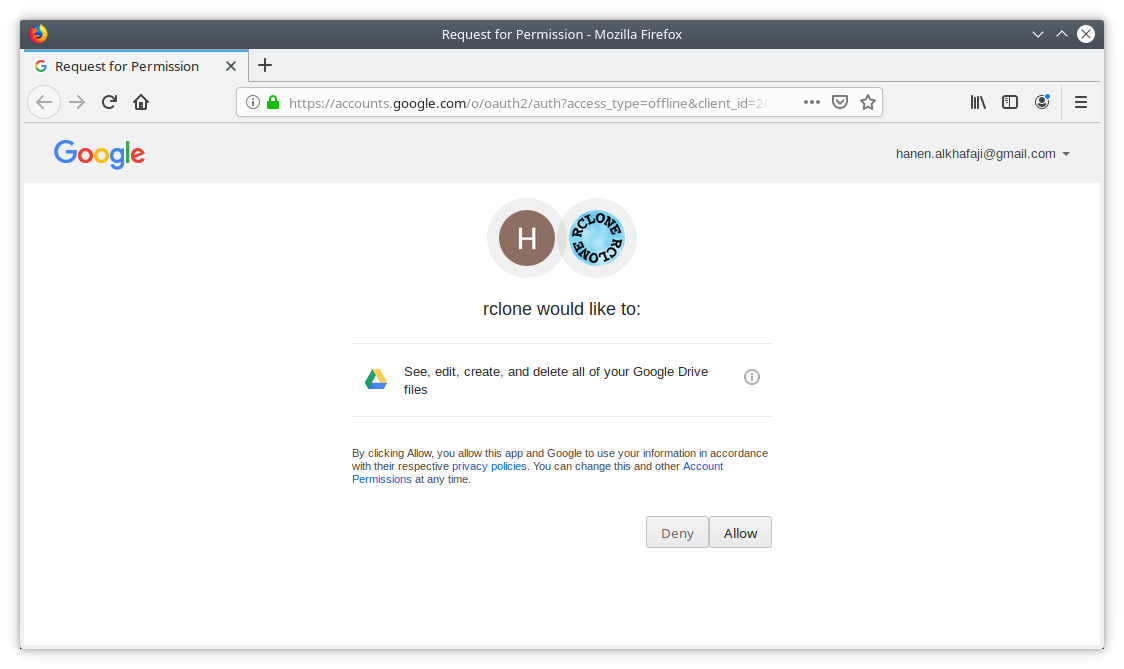
\includegraphics[scale=0.4]{images/rclone1.png}
  \caption{First RClone Screenshot}
  \label{fig:rclone1}
\end{figure}

\begin{figure}[htb]
  \centering
  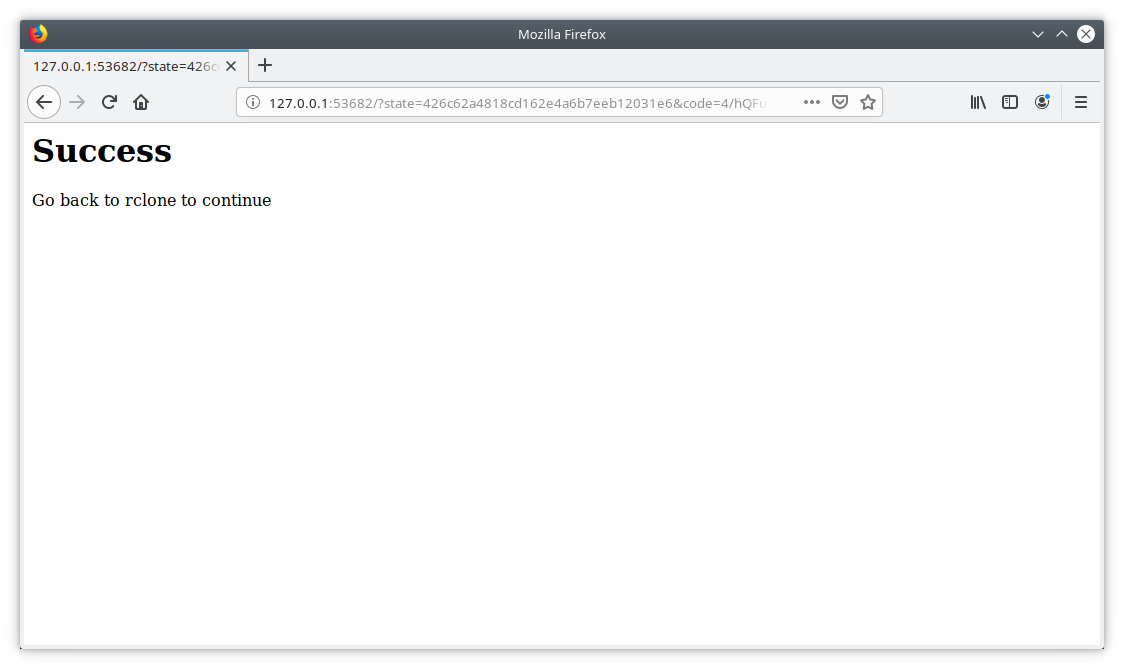
\includegraphics[scale=0.4]{images/rclone2.png}
  \caption{Second RClone Screenshot}
  \label{fig:rclone2}
\end{figure}

\begin{verbatim}
    If your browser doesn't open automatically go to the following 
    link: http://127.0.0.1:53682/auth
    Log in and authorize rclone for access
    Waiting for code...
    Got code
    Configure this as a team drive?
    y) Yes
    n) No
    y/n> n
    --------------------
    [remote]
    client_id = 
    client_secret = 
    scope = drive
    root_folder_id = 
    service_account_file = 
    token = {"access_token":"ya29.GltEB013ECs9MfyyGMcUfoSt_zNOt5
    jhU0bd7iON_VHep0cqyIVXC211TkJ1hdyKFEPb98rBKznYaGP1aoF4xIkHHBi
    5O8Gre6t4VpwVX06wGZkEELEr3sxzeu2L","token_type":"Bearer",
    "refresh_token":"1/TQ9fv-iDU4NqZkM5hngLF01tDhRfrtm_XKbDRdfarR8",
    "expiry":"2019-07-13T00:24:12.763120806-04:00"}
    --------------------
    y) Yes this is OK
    e) Edit this remote
    d) Delete this remote
    y/e/d> y
    Current remotes:
    
    Name                 Type
    ====                 ====
    remote               drive
    
    e) Edit existing remote
    n) New remote
    d) Delete remote
    r) Rename remote
    c) Copy remote
    s) Set configuration password
    q) Quit config
    e/n/d/r/c/s/q> q
    hanen@hanen:~$ rclone lsd remote:
              -1 2019-06-19 22:53:37        -1 2019-Hanen-CS-6970
              -1 2019-06-04 10:46:41        -1 Misc
\end{verbatim}

\subsection{Android Tablet}
\label{rclonegdrivedemo}

As in the Linux Machine section above, the same commands are used on the Android device. In order to run commands, the Termux app must be installed from the Google Play Store. I struggled for awhile to get past some permission issues until I discovered a very helpful YouTube video \cite{youtubetermux}, which helped me overcome this obstacle. \\ \\
I used the steps from a GitHub page \cite{rclonetermux} to setup RClone on the Android tablet using Termux. It behaved exactly the same way with the exception of a few additional prompts that I was expected to interact with compared to the Linux machine. I responded to these additional prompts by simply pressing Enter without providing any input. This results in the application using the defaults. The following are the prompts I got before the browser popped up asking for permissions: \\ \\
    \verb|service_account_credentials|\\
    \verb|auth_owner_only|\\
    \verb|use_trash|\\
    \verb|skip_gdocs|\\
    \verb|skip_checksum_gphotos|\\
    \verb|shared_with_me|\\
    \verb|trashed_only|\\
    \verb|formats|\\
    \verb|export_formats|\\
    \verb|import_formats|\\
    \verb|allow_import_name_change|\\
    \verb|use_created_date|\\
    \verb|list_chunk|\\
    \verb|impersonate|\\
    \verb|alternate_export|\\
    \verb|upload_cutoff|\\
    \verb|chunk_size|\\
    \verb|acknowledge_abuse|\\
    \verb|keep_revision_forever|\\
    \verb|size_as_quote|\\
    \verb|v2_download_min_size|\\
    \verb|pacer_min_sleep|\\
    \verb|pacer_burst|\\
    \verb|server_side_across_configs|
\section{ODrive}
\section{InSync}
\begin{figure}[htb]
  \centering
  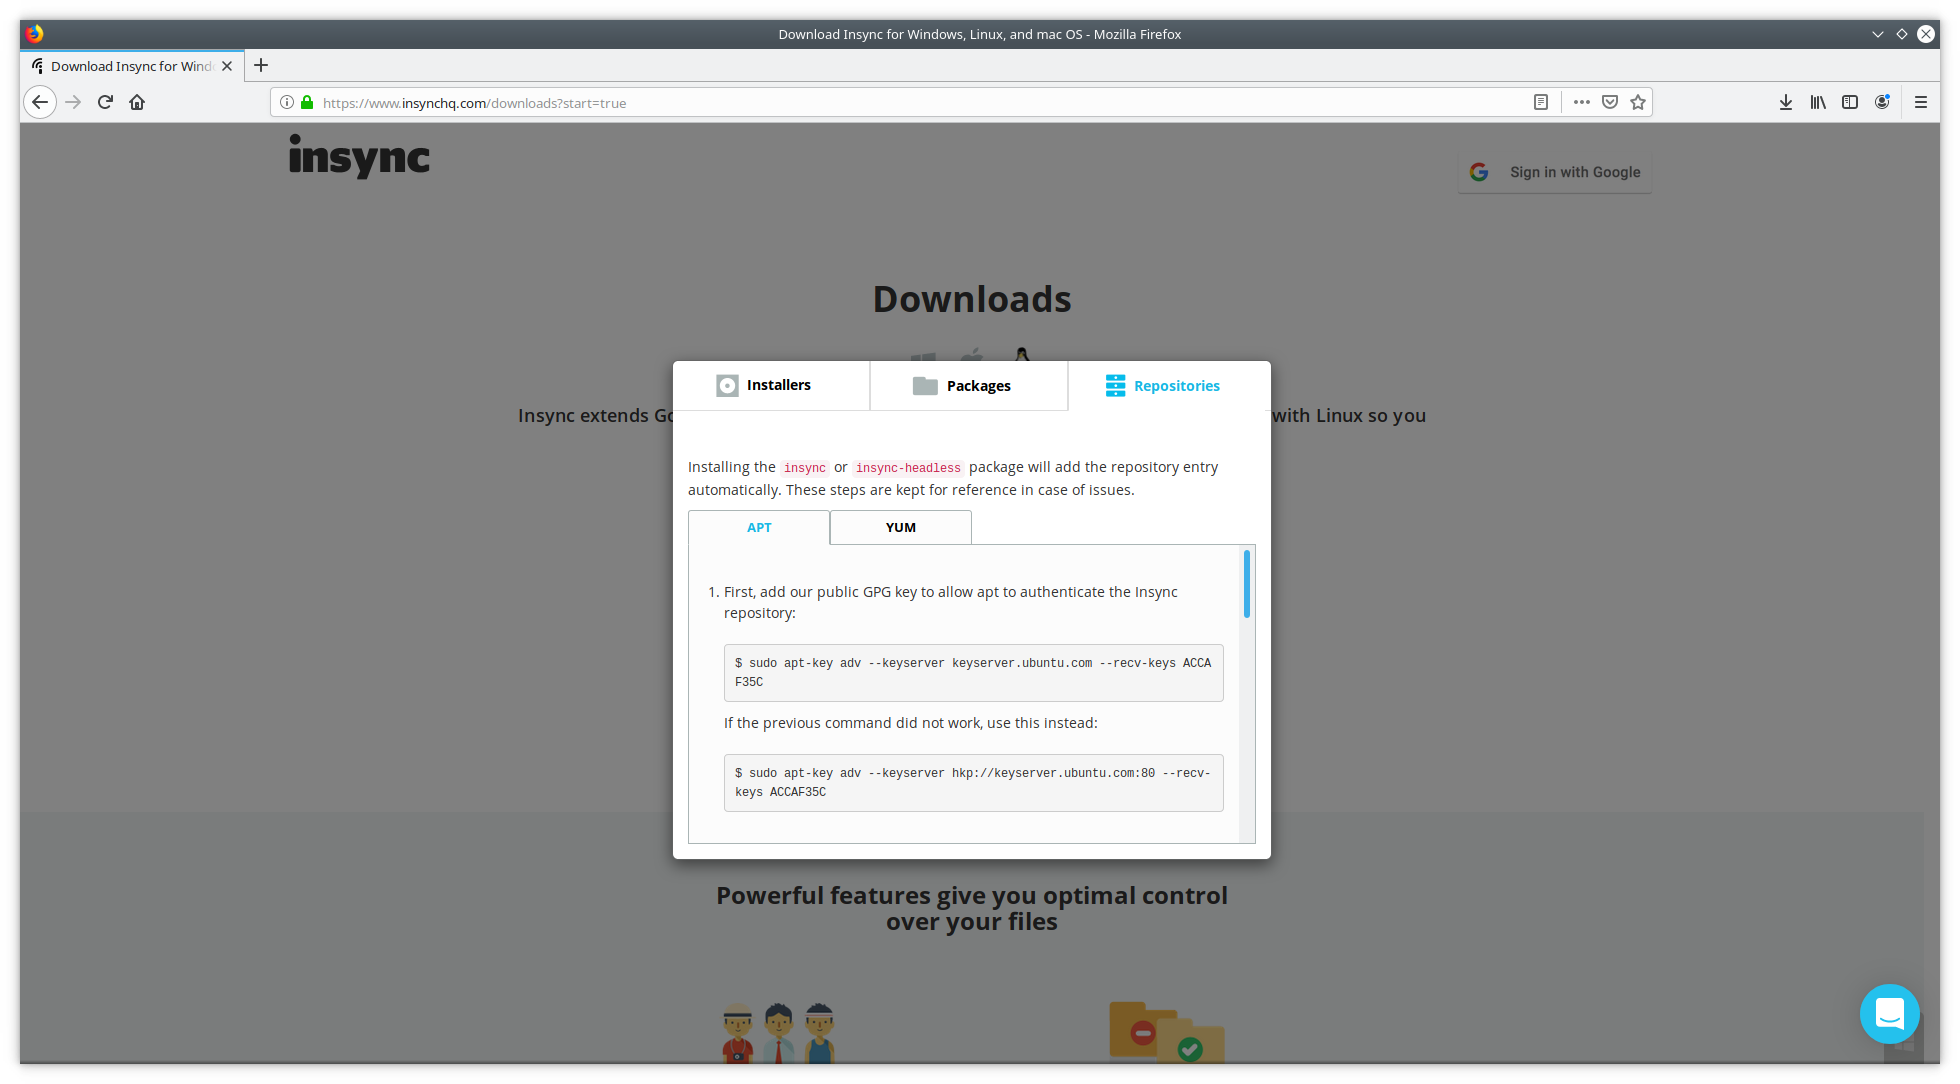
\includegraphics[scale=0.2]{images/insync0.png}
  \caption{Install Instructions on InSync Website}
  \label{fig:insync0}
\end{figure}
Following the instructions on the InSync website as illustrated in Figure \ref{fig:insync0}, the following commands were executed in order to install InSync and sync a folder from Google Drive to a folder on the Linux machine's local drive. \cite{insync}
\begin{verbatim}
root@hanen:/mnt# sudo apt-key adv --keyserver keyserver.ubuntu.com 
--recv-keys ACCAF35C
Executing: /tmp/apt-key-gpghome.8tQidnAcU1/gpg.1.sh 
--keyserver keyserver.ubuntu.com --recv-keys ACCAF35C
gpg: key A684470CACCAF35C: public key "Insynchq Inc 
<services@insynchq.com>" imported
gpg: Total number processed: 1
gpg:               imported: 1
root@hanen:/mnt# lsb_release -a
No LSB modules are available.
Distributor ID: Ubuntu
Description:    Ubuntu 18.10
Release:        18.10
Codename:       cosmic
root@hanen:/mnt# echo "deb http://apt.insynchq.com/ubuntu cosmic 
non-free contrib" >> /etc/apt/sources.list.d/insync.list
root@hanen:/mnt# sudo apt-get update
Hit:1 http://security.ubuntu.com/ubuntu cosmic-security InRelease
Hit:2 http://packages.microsoft.com/repos/vscode stable InRelease                                          
Hit:3 http://us.archive.ubuntu.com/ubuntu cosmic InRelease                                                 
Ign:4 http://packages.cloud.google.com/apt gcsfuse-cosmic InRelease                                        
Hit:5 http://ppa.launchpad.net/alessandro-strada/ppa/ubuntu cosmic 
InRelease                   
Hit:6 http://us.archive.ubuntu.com/ubuntu cosmic-updates InRelease                                         
Err:7 http://packages.cloud.google.com/apt gcsfuse-cosmic Release                                          
  404  Not Found [IP: 172.217.14.174 80]
Hit:8 http://us.archive.ubuntu.com/ubuntu cosmic-backports InRelease                                       
Get:9 http://apt.insynchq.com/ubuntu cosmic InRelease [5,557 B]                                            
Hit:10 http://ppa.launchpad.net/avsm/ppa/ubuntu cosmic InRelease                                           
Get:11 http://apt.insynchq.com/ubuntu cosmic/non-free amd64 
Packages [776 B]
Get:12 http://apt.insynchq.com/ubuntu cosmic/non-free i386 
Packages [619 B]
Get:13 http://apt.insynchq.com/ubuntu cosmic/contrib i386 
Packages [1,253 B]
Get:14 http://apt.insynchq.com/ubuntu cosmic/contrib amd64 
Packages [1,579 B]
Reading package lists... Done      
E: The repository 'http://packages.cloud.google.com/apt gcsfuse-cosmic 
Release' does not have a Release file.
N: Updating from such a repository can't be done securely, and is 
therefore disabled by default.
N: See apt-secure(8) manpage for repository creation and user 
configuration details.
root@hanen:/mnt# sudo apt-get install insync
Reading package lists... Done
Building dependency tree       
Reading state information... Done
The following packages were automatically installed and are no 
longer required:
  libncursesw5 libtinfo5
Use 'sudo apt autoremove' to remove them.
The following NEW packages will be installed:
  insync
0 upgraded, 1 newly installed, 0 to remove and 10 not upgraded.
Need to get 144 MB of archives.
After this operation, 400 MB of additional disk space will be used.
Get:1 http://apt.insynchq.com/ubuntu cosmic/non-free amd64 insync 
amd64 1.5.7.37371-artful [144 MB]
Fetched 144 MB in 39s (3,678 kB/s)                                                                         
Selecting previously unselected package insync.
(Reading database ... 230974 files and directories currently 
installed.)
Preparing to unpack .../insync_1.5.7.37371-artful_amd64.deb ...
Unpacking insync (1.5.7.37371-artful) ...
Processing triggers for mime-support (3.60ubuntu1) ...
Setting up insync (1.5.7.37371-artful) ...
Insync installation has finished. You may now start it.
Insync doesn't seem to be running. Start it first.

fs.inotify.max_user_watches = 1048576
Processing triggers for man-db (2.8.4-2) ...
Processing triggers for shared-mime-info (1.10-1) ...
Processing triggers for hicolor-icon-theme (0.17-2) ...
\end{verbatim}
Once the install is complete, the InSync pop-ups appear guiding the user through the setup process. The welcome screen appears giving the user the chance to add a Google account for syncing as illustrated in Figure \ref{fig:insync1}. Once that button is clicked, a browser appears allowing the user to choose which account to sync followed by a screen requesting access to that account as illustrated in Figure \ref{fig:insync2}. Once access is granted, a screen appears letting the user know that the handshake is complete as illustrated in Figure \ref{fig:insync3}. InSync, then, creates a folder for the newly connected drive as illustrated in Figure \ref{fig:insync4}. If the user confirms this action, the following screen lets the user begin syncing either all or select folders as illustrated in Figure \ref{fig:insync5}. \\
\begin{figure}[htb]
  \centering
  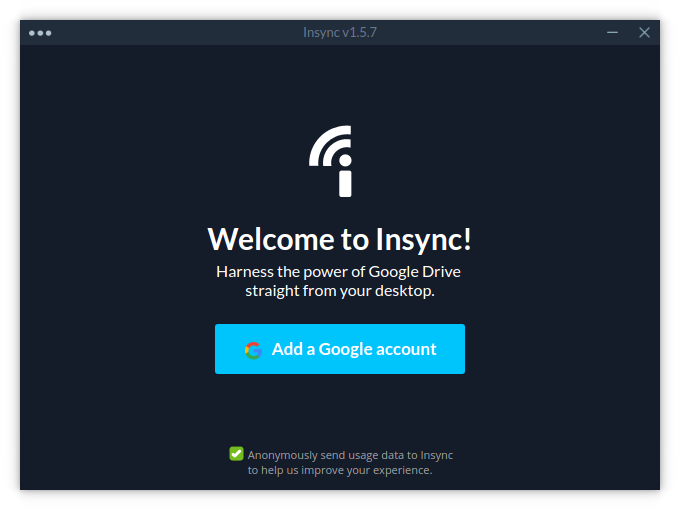
\includegraphics[scale=0.4]{images/insync1.png}
  \caption{InSync Welcome Screen}
  \label{fig:insync1}
\end{figure}
\begin{figure}[htb]
  \centering
  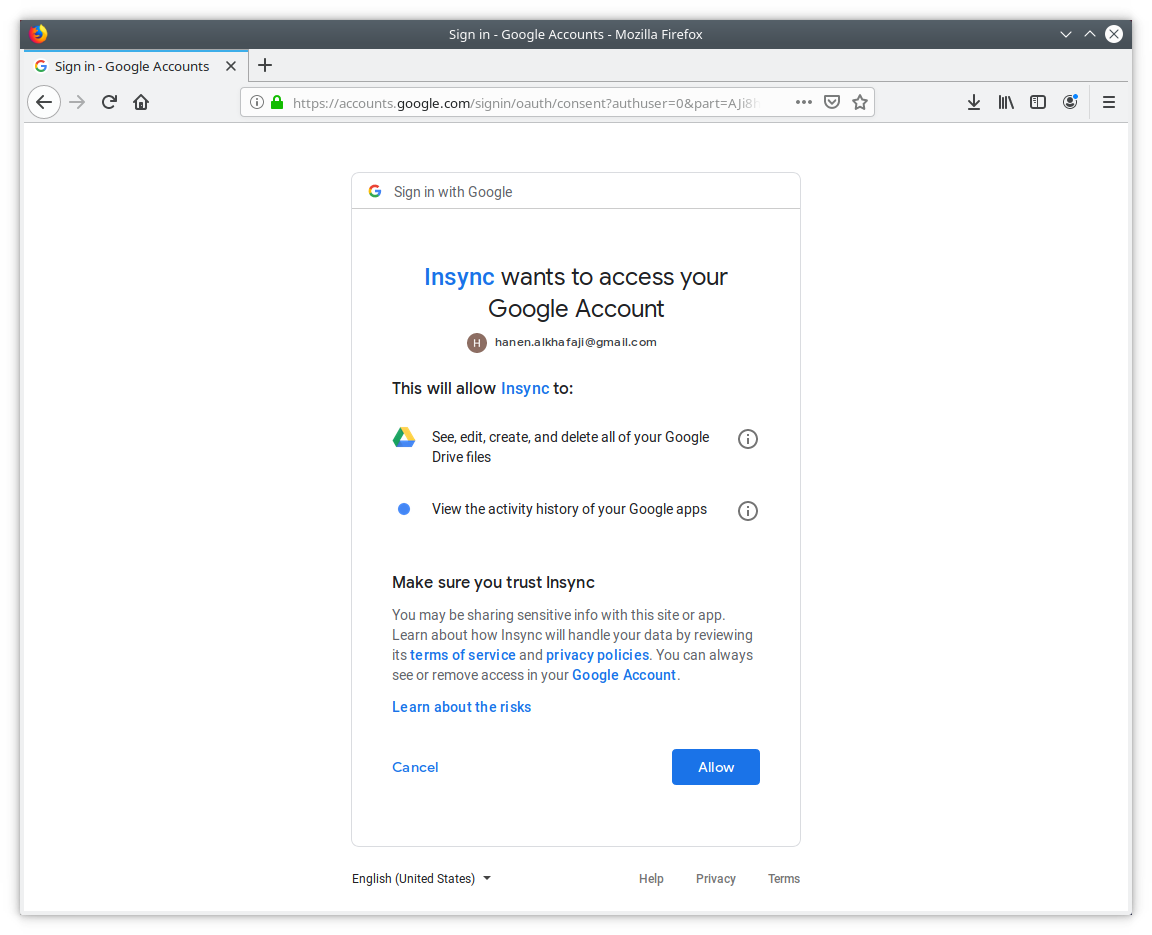
\includegraphics[scale=0.4]{images/insync2.png}
  \caption{InSync Requests Access}
  \label{fig:insync2}
\end{figure}
\begin{figure}[htb]
  \centering
  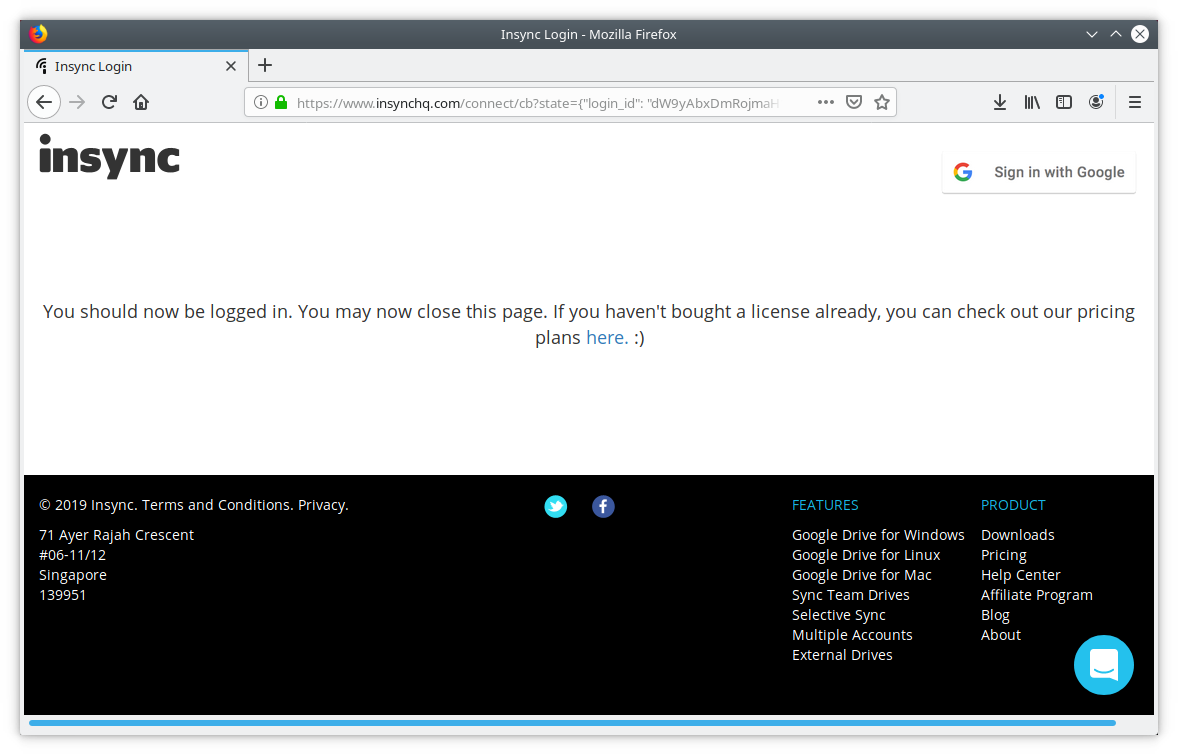
\includegraphics[scale=0.4]{images/insync3.png}
  \caption{InSync Installation Complete}
  \label{fig:insync3}
\end{figure}
\begin{figure}[htb]
  \centering
  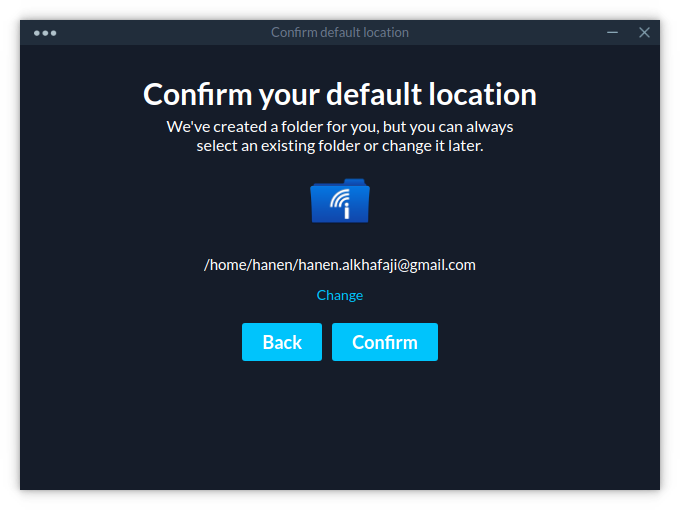
\includegraphics[scale=0.4]{images/insync4.png}
  \caption{InSync created folder for syncing Google Drive}
  \label{fig:insync4}
\end{figure}
\begin{figure}[htb]
  \centering
  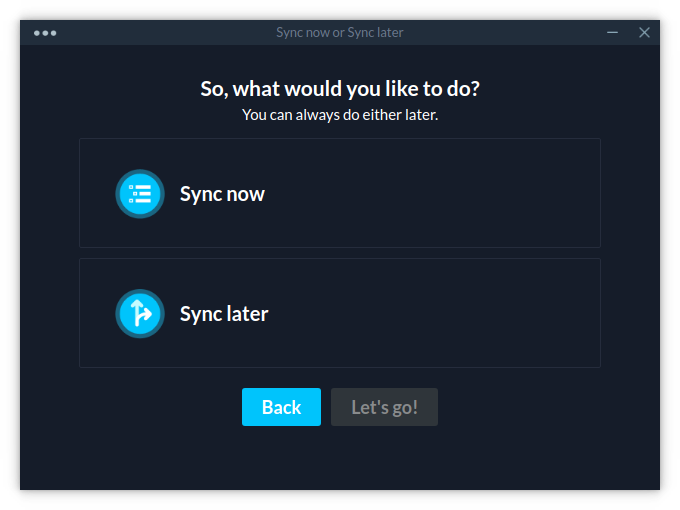
\includegraphics[scale=0.4]{images/insync5.png}
  \caption{InSync is ready to sync folders}
  \label{fig:insync5}
\end{figure}
As a result, the following appears in the terminal.
\begin{verbatim}
root@hanen:~/hanen.alkhafaji@gmail.com# ls
2019-Hanen-CS-6970
\end{verbatim}

\section{X-Plore}

\section{Write FileSystem with FUSE}

\section{ES File Explorer}

\section{Mounting using SSHFS}


%==============================================================================================================================================
\chapter{Meeting Minutes}
\label{meetingminutes}
\section{5/14/2019}
This initial meeting of the summer involved discussions and decisions around which project I should tackle for the independent study course. Dr. Mateti presented two topics we had discussed in meetings prior to this initial one. These two topics were selected after we had discussed other options and narrowed them down to a project dealing with Cloud Computing and a project dealing with Cloud Storage. Both projects would involve Android. The Cloud Computing topic would be one in which I would research different cloud computing approaches. The Cloud Storage topic would involve implementing a solution for mounting different cloud storage folders onto an Android device at the operating system level. There are many apps available that will do this very thing on the application level, where a user interacts with their cloud storage through the application itself, but cannot access that mounted storage from any other app on the device. Dr. Mateti showed me some apps like that on his phone which included ES File Explorer and X-plore. The goal would be mounting the storage at the OS level so that the user can access it from any app as if it were simply just another folder on their Android file system.\\ \\
I decided to select the topic of Cloud Storage, because I really wanted to implement something this summer and this sounded both interesting and personally useful. Once I selected the topic I wanted to focus on, Dr. Mateti elaborated further on expectations and next steps. We will meet in his office at 6pm on Tuesdays or Thursdays on an as-needed basis. In the meantime, I will be uploading my meeting minutes and technical document drafts to a shared Google Drive folder that Dr. Mateti has been given access. I will, also, be organizing the tasks needed to accomplish this project using an application called Trello. Dr. Mateti has been given access to this board on Trello. The technical document will be around 50 pages once it is complete and will use Software Engineering principles. I was tasked to explore open source options for mounting Google Cloud and/or Firebase. Other things to read about and look into included Fuse and SSHFS. The plan will be to implement any solution on a Linux PC first. Then, when it is working to our satisfaction, it will be ported over to Android. \\ \\
Dr. Mateti also provided me with an Android tablet to be used for this course. I will be bringing back the other tablet I borrowed in our next meeting.
\section{6/4/2019}
Dr. Mateti and I met to primarily discuss the development plan for my project for the summer. The goal for the summer is to be able to demonstrate mounting Google Drive at the operating system level on an Android device. The secondary goal is to try the same for another cloud storage provider, but we will determine later if we have time for that. \\ \\
On KDE, I need to install GDrive (KIO). There is an authentication error that appears that can be resolved by going into System Settings and adding an Online Account for Google Drive. There was also another error that could be resolved by going into Personal Settings and enabling the KDE Wallet. If all else fails, remove the account under System Settings and add it back. \\ \\
Dr. Mateti provided some helpful hints on using Latex such as \texttt{\tt} for using a typewriter script to distinguish a certain chunk of text from the remaining report. \verb|\begin{verbatim}| terminal output \verb|\end{verbatim}| was another helpful tip. \\ \\
Dr. Mateti also provided me with a usb input cable that I will use to create a DIY OTG cable, so that I can plug a USB into my tablet. I will plug the USB into my tablet and mount it using the code I develop. \\ \\
Some action items that Dr. Mateti sent me away with were:
\begin{enumerate}
\item Put together a Development Plan document.
\item Revisit the init lab from the Android Security and Internals course from last semester.
\item Browse the OCamlFUSE code and determine comfort level with using it. Do lab report.
\item Rclone might be able to do mounting at the OS level and can handle more cloud storage providers. Do lab report. Include SLOC count of source code.
\item Odrive. Do lab report.
\item InSync. Try the free trial. Do lab report.
Do lab report on mounting a USB drive.
\end{enumerate}
\section{6/11/2019}
Dr. Mateti provided me with a tablet that has already been rooted. This will help me make progress without the risk of bricking the device like I did before. Dr. Mateti reviewed his feedback to my OCamlFUSE lab report. He shared a Latex format he would like me to use for my final report. He asked me to mount a usb drive using an OTG cable. He, also, asked that I make some changes to an existing OCaml project. The plan is to focus on these two items. The feedback given by Dr. Mateti was uploaded on Google Drive. I will need to upload the Latex files he provided and fill things in based on his suggestions.
\section{7/30/2019}
I met with Dr. Mateti to discuss wrapping up the semester and this project. Due to the issues we have run into with OPam to build the OCamlFUSE solution, we have decided to turn our attention to RClone instead. I need to include a section in this report about Android internals and what current applications do with regard to syncing cloud storage. I need to, also, demonstrate RClone on Android to mount four different cloud storage providers. I need to explain in the conclusion what I've learned, what I did, why FUSE, why OCaml, and what future work needs to be done if time were not limited. I need to explain what went wrong with OCamlFUSE like issues with the OPam.

%==============================================================================================================================================
\chapter{Schedule and Activities}
\label{schedule}

\begin{itemize}
  \item May 14: Decide on project topic
  \item May 14: On Campus Meeting
  \item May 17: Read about Fuse
  \item May 21: Read about SSHFS
  \item May 21: Install and Try ES File Explorer
  \item May 23: Install and Try X-plore
  \item May 23: Draft 1
  \item June 2: Learned LaTeX and Converted Report
  \item June 3: Project Scope Document
  \item June 4: On Campus Meeting
  \item June 6: Draft 2
  \item June 8: OCamlFUSE Mount on Linux
  \item June 11: Dr. Mateti provides rooted Nexus 7 tablet
  \item June 11: On Campus Meeting
  \item June 13: Cloud Storage Mounts in Android
  \item June 17: Lab Report: OCamlFUSE
  \item June 18: Make Changes to Sample Code
  \item June 20: Draft 3
  \item June 21: Create Outline to Guide Project
  \item June 23: Mount USB
  \item July 24: Draft 4
  \item August 5: Final Technical Report
\end{itemize}

